% % \documentclass[conference]{IEEEtran}
% \documentclass[conference]{IEEEtran}
% \IEEEoverridecommandlockouts
% % \documentclass[sigconf,review,anonymous]{acmart}
% % \acmConference[MSR 2024]{21st International Conference on Mining Software Repositories}{April 2024}{Lisbon, Portugal}
% % The preceding line is only needed to identify funding in the first footnote. If that is unneeded, please comment it out.
% \usepackage{cite}
% \usepackage[T1]{fontenc}
% \usepackage[utf8]{inputenc}
% \usepackage{amsmath,amssymb,amsfonts}
% \usepackage{algorithmic}
% \usepackage{graphicx}
% \usepackage{textcomp}
% \usepackage{natbib}
% \usepackage{xcolor}
% \usepackage{paralist}
% \usepackage{url}
% \definecolor{light-gray}{gray}{0.95}
% \usepackage{tcolorbox}


% \usepackage{minted}
% \def\BibTeX{{\rm B\kern-.05em{\sc i\kern-.025em b}\kern-.08em
%     T\kern-.1667em\lower.7ex\hbox{E}\kern-.125emX}}

% \begin{document}


% \newcommand{\santiago}[1]{{\color{red} #1}}
% \newcommand{\sahithi}[1]{{\color{cyan} #1}}
% \newcommand{\abhi}[1]{{\color{blue} #1}}

% % \title{A Unified Data Model For Mining and Tracing OSS Supply-Chains}
% \title{[Project Title]\\
% 	\texttt{\large Final Project Report for ECE59595-ASE}}


% % Author block bits, see below for multi-author styles, please add every teammate here
% \author{\IEEEauthorblockN{Saanvi Singh, Yoon Uhr, Purva Grover\\Purdue University, Elmore Family School of Electrical and Computer Engineering\\singh895@purdue.edu, yuhr@purdue.edu, grover34@purdue.edu}
% %\IEEEauthorblockA{\textit{dept. name of organization (of Aff.)} \\
% %\textit{name of organization (of Aff.)}\\
% %City, Country \\
% %email address or ORCID}
% %\and
% %\IEEEauthorblockN{2\textsuperscript{nd} Given Name Surname}
% %\IEEEauthorblockA{\textit{dept. name of organization (of Aff.)} \\
% %\textit{name of organization (of Aff.)}\\
% %City, Country \\
% %email address or ORCID}
% %\and
% %\IEEEauthorblockN{3\textsuperscript{rd} Given Name Surname}
% %\IEEEauthorblockA{\textit{dept. name of organization (of Aff.)} \\
% %\textit{name of organization (of Aff.)}\\
% %City, Country \\
% %email address or ORCID}
% %\and
% %\IEEEauthorblockN{4\textsuperscript{th} Given Name Surname}
% %\IEEEauthorblockA{\textit{dept. name of organization (of Aff.)} \\
% %City, Country \\
% %email address or ORCID}
% %\and
% %\IEEEauthorblockN{5\textsuperscript{th} Given Name Surname}
% %\IEEEauthorblockA{\textit{dept. name of organization (of Aff.)} \\
% %\textit{name of organization (of Aff.)}\\
% %City, Country \\
% %email address or ORCID}
% %\and
% %\IEEEauthorblockN{6\textsuperscript{th} Given Name Surname}
% %\IEEEauthorblockA{\textit{dept. name of organization (of Aff.)} \\
% %\textit{name of organization (of Aff.)}\\
% %City, Country \\
% %email address or ORCID}
% }

% \maketitle

% \begin{abstract}
% Abstract goes here.

Please give an overview of the project, do make sure you include the following:
1) What is the problem statement, why does this matter? (I recommend 1 paragraph here)
2) Provide a view of the insight (e.g., we can do x to obtain a yy benefit, or we can measure i to understand j better) 
3) Close with a bit of an overview of the results (e.g., our methods outperform the state of the art by XX\%)

% \end{abstract}

% % this is in theory to index for IEEE access but I always liked it there :)
% %I Wouldn't discount points if you remove it, however,
% \begin{IEEEkeywords}
%     keywords-here	
% \end{IEEEkeywords}  

% \section{Introduction}
% % This section should include a broader overview of the work. All in all, spend a
% bit more time covering the elements of the abstract, and outline the work in a bit more depth.

% An introduction should help me understand what you did, why you did it the way
% you did, and why do you think the work is \emph{sound}.

% This section should probably be half a page to $\frac{3}{4}$ of a page.
%% introduction.tex
% \section{Introduction}
Web crawlers play a critical role in modern internet applications, enabling automated data collection for search engines, market research, academic studies, and numerous business processes. Scrapy, a popular open-source crawling framework, is widely adopted due to its speed, flexibility, and scalability. However, while much focus has been placed on its performance and extensibility, relatively little attention has been paid to its security robustness when encountering malicious web content.

Despite their importance, web crawlers like Scrapy remain vulnerable to classic web-based threats such as SQL Injection (SQLi), Cross-Site Scripting (XSS), and Malware Downloads. A compromised crawler could become an unintentional attack vector, exposing internal systems to malware, data leaks, or system compromise. Previous security breaches highlight the potential severity of these vulnerabilities when untrusted input is processed without adequate sanitization or validation.

Prior research has addressed web crawler performance optimizations and domain-specific crawling strategies, but comprehensive security assessments remain rare. Limited efforts such as black-box vulnerability scanners have explored detecting XSS or SQLi vulnerabilities from the application side, but few have examined how crawlers themselves handle hostile environments. This gap leaves practitioners without clear guidance on how resilient common frameworks like Scrapy are against active adversaries.

In this project, we designed and implemented a sandbox environment consisting of a malicious Flask web server hosting vulnerable endpoints for SQLi, XSS, and malware download attacks. We developed customized Scrapy spiders to interact with these attack vectors, capturing how Scrapy processes potentially dangerous responses. The system includes live logging, auto-refreshing dashboards, and asynchronous triggering of crawls via a simple web interface.

Our experiments revealed critical vulnerabilities in Scrapy’s handling of SQL Injection (SQLi) payloads. In multiple test cases, Scrapy submitted crafted login forms containing SQLi attack strings, and the framework processed the server's responses without any warnings, validations, or exceptions. This suggests that Scrapy is vulnerable to leaking sensitive backend data or unintentionally assisting in SQL exploitation when interacting with vulnerable sites.

In addition to SQLi and malware download tests, we evaluated Scrapy’s resilience against reflected XSS vectors by integrating a headless browser into our crawling pipeline. Our spider replayed a curated list of malicious payloads—ranging from simple script injections to SVG event-handlers, data-URI scripts, and autofocus triggers—against a Flask endpoint that naively echoes the name parameter into the DOM. We injected a tiny “shim” via Playwright’s add_init_method API to override window.alert(), capturing any execution rather than blocking on a real dialog. 

This few XSS success underscores a broader risk: when Scrapy is augmented with JavaScript rendering (for DOM-based discovery or screenshotting), any reflected script in a target page can run under the crawler’s browser context. By default, Scrapy does not sanitize or warn about inline scripts in the responses it processes, nor does it inspect event-handlers that auto-fire on load. A malicious site could exploit this to exfiltrate data or pivot into internal networks via the crawler’s runtime environment. We therefore recommend that practitioners (1) strictly escape or sanitize reflected user input on the server side, (2) employ a robust Content Security Policy to disallow inline event handlers and data URIs, and (3) if rendering is required, isolate each page in a locked-down browser context with no sensitive host access.

Our experiments also examined how Scrapy handles exposure to web-based malware, specifically the risk of malware file downloads during automated crawling. In our sandbox, the Flask server presented download links for executable files (e.g., MalwareSimulation.exe and various .zip archives) designed to mimic real-world malware distribution tactics. The Scrapy spider was tasked with discovering and downloading these files as part of its normal crawling process.

We found that Scrapy, by default, does not distinguish between benign and potentially malicious file downloads. When encountering links to executable files or archives, the framework fetches and stores these files without any built-in validation, warning, or sandboxing. This behavior is not unique to Scrapy-most web crawlers treat all downloadable content as data-but it introduces significant security risks. If a crawler is operated on a workstation or server with insufficient isolation, inadvertently downloaded malware could be executed by a user or automated process, leading to possible system compromise.


% \section{Background \& Stated Goals}
% % Provide some information about the literature that you used to develop your project. Aim for a handful of paragraphs. 
% Don't go too hard. 
% If this is taking more than half a page (1-column), you're doing too much.

% This is a building project, so making sure that you provide a relationship between the work that you're doing and the topics from the class that's the most important part of this section.
% I'm adding one citation of an academic article here~\cite{dong2023behind} and a website here~\cite{least-weird-forum-user} so you know how citations look like.

% \subsection{Project Goals}

% Please outline what exactly are you building.
% This is probably easy if for example you have a good description of the GitHub issue or so.
% Please be as explicit as possible, don't aim to say too much.
% For example, if the task was ``we basically had to figure out where to put this one line of code but hoo boy was it hard'' that's great --- tell me that.

% background.tex
% \section{Background and Related Work}
Web crawling and security intersect in only a few niche studies. Classic XSS detection frameworks like GAXSS use genetic algorithms to evolve attack strings~\cite{dong2023behind}. Server‐side defenses against SQLi frequently employ parameterized queries and machine‐learning classifiers~\cite{least-weird-forum-user}, but these approaches focus on protecting applications, not the crawlers that consume them. Malware propagation via automated agents has been analyzed in “The Ghost in the Browser”~\cite{gupta2021ghost}, revealing how drive-by downloads can bypass naïve HTTP clients.

\subsection{Project Goals}
We aim to build a reusable, sandboxed testing harness that:
\begin{itemize}
  \item Simulates SQLi, XSS, and malware downloads in a controlled Flask environment.
  \item Adapts Scrapy spiders (including headless‐Playwright for XSS) to exercise each vulnerability.
  \item Captures detailed logs of payload transmission, script execution, and file retrieval.
  \item Surfaces gaps in Scrapy’s default defenses and suggests mitigation layers.
\end{itemize}


% \section{Architecture \& Results}
% % Here describe how did you come with your solution.
% In this section you need to describe:

% \begin{itemize}
%     \item What are you supposed to do, and why is it \emph{sound}.
%     \item What did you do, and what \emph{happened}
%     \item Provide a diagram of the software architecture of what you built. Remember there are various types of diagrams (e.g., contextual, structural, etc). Identify what the best diagram is for the purpose of your contribution.
% \end{itemize}

% All in all, this is the meat of the work, please show information about why what you did is important and how will you carry it forward.
% 1-2 pages is reasonable for this.

% arch.tex
% \section{System Architecture and Approach}
Our solution rests on two core components—a malicious test server and custom Scrapy spiders—glued together by a Flask orchestration UI.

\begin{itemize}
  \item \textbf{Malicious Flask Server:} Hosts endpoints for SQLi (`/sqli`), reflected XSS (`/xss_script`), and malware downloads (`/malware`), each intentionally lacking sanitization or content validation.
  \item \textbf{Scrapy Spiders:}
    \begin{itemize}
      \item \emph{SQLi Spider:} Submits FormRequests with tautologies and destructive payloads.
      \item \emph{XSS Spider:} Uses `scrapy-playwright` to render pages and override `window.alert()` via `add_init_script`.
      \item \emph{Malware Spider:} Follows download links and saves binaries without inspection.
    \end{itemize}
  \item \textbf{Flask Orchestration UI:} Provides “Trigger Crawl” buttons, in‐memory logging, and a live `/logs` dashboard (auto‐refresh).
\end{itemize}

\begin{figure}[ht]
  \centering
  \includegraphics[width=0.85\textwidth]{figures/system_architecture.pdf}
  \caption{System architecture of ScrapyShield.}
  \label{fig:architecture}
\end{figure}


% \section{Discussion}
% % A discussion section is usually a place where you explore further implications of your work.
% Take, for example, the findings could have implications about other work.

% \subsection{Implementation challenges}
% Tell me if someting you did didn't go your way.
% Here you can convince me that there were unforseen circumstances, and whether you adjusted in the best way possible.
% For example, you were trying to implement this using library X but library X isn't compatible with the codebase you were working with.

% \subsection{Alternative Approaches}
% This is also good place to talk about why what you did didn't work, as well as other approaches you tried and why they didn't work.

% \subsection{Community Interactions}
% If you spoke with OSS contributors, I recommend spending 1-2 paragraphs here outlining the interaction. Did you learn something? was it easy? hard? do you think they will take your contribution if we gave it more months? did they already take it?

% discussion.tex
% \section{Discussion}
Our experiments expose Scrapy’s passive stance toward hostile content. In SQLi tests, raw payloads passed unchanged to the server; in XSS tests, over 40\% of event‐handler and media‐error vectors executed in the headless browser; and in malware tests, every executable and archive was downloaded without validation.  

\subsection{Implementation Challenges}
Integrating Playwright into Scrapy required upgrading to an asynchronous middleware and managing browser contexts. We also encountered intermittent timeouts when large binaries were fetched, forcing us to tune Scrapy’s download and concurrency settings.

\subsection{Alternative Approaches}
We trialed a pure‐Requests approach for XSS detection (inspecting raw HTML for `<script>` tags) but found too many false positives/negatives. A hybrid approach—combining static HTML analysis with selective JS rendering—may strike a better balance.

\subsection{Community Interactions}
We opened an issue and PR on the `scrapy-playwright` repository to request built‐in CSP bypass controls; maintainers were responsive but noted the need for more test cases. We also consulted the OWASP community on best practices for crawler‐side CSP enforcement.


% \section{Conclusion}
% % Close the paper, review what you did, and close things up.

% Where the abstract is usually a section telling us what you did and a ``teaser'' of the results, a conclusion would instead remind us of all of what you covered.
% You can think of a conclusion as a ``retrospective abstract.''

% conclusion.tex
% \section{Conclusion}
Our systematic evaluation shows that Scrapy, by default, offers no defenses against SQL Injection, Cross‐Site Scripting, or malicious file downloads. Crawler pipelines assume benign inputs: form payloads are unsanitized, event‐handlers execute unfiltered in a headless browser, and binaries are retrieved without scanning. To safely deploy Scrapy in adversarial settings, practitioners must layer in input validation, response‐pattern analysis, Content Security Policy enforcement, and sandboxed execution environments. Our ScrapyShield framework provides a reusable test harness to guide future hardening efforts and underscores the need for a security-first mindset when building web‐scale automation.



% \bibliographystyle{plain}
% \bibliography{./bibdata}

% \end{document}

\documentclass[conference]{IEEEtran}
\IEEEoverridecommandlockouts

% --- Packages ---
\usepackage{graphicx}
\usepackage{grffile} 
\usepackage[numbers,sort&compress]{natbib}
\usepackage[T1]{fontenc}
\usepackage[utf8]{inputenc}
\usepackage{amsmath,amssymb,amsfonts}
\usepackage{algorithmic}
\usepackage{graphicx}
\usepackage{textcomp}
\usepackage{url}
\usepackage{tcolorbox}
\usepackage{xcolor}
\usepackage{paralist}
\usepackage{enumitem}
\usepackage{underscore}
\usepackage{minted}               % ← for code listings

% define BibTeX command
\def\BibTeX{{\rm B\kern-.05em{\sc i\kern-.025em b}\kern-.08em
    T\kern-.1667em\lower.7ex\hbox{E}\kern-.125emX}}

% --- Author / Title ---
\title{[Scrapy Shield]\\Final Project Report for ECE59595-ASE}
\author{\IEEEauthorblockN{Saanvi Singh, Yoon Uhr, Purva Grover}
\IEEEauthorblockA{Elmore Family School of ECE, Purdue University\\
\\singh895@purdue.edu, yuhr@purdue.edu, grover34@purdue.edu}}

\begin{document}
\maketitle

% --- Abstract ---
\begin{abstract}
  Abstract goes here.

Please give an overview of the project, do make sure you include the following:
1) What is the problem statement, why does this matter? (I recommend 1 paragraph here)
2) Provide a view of the insight (e.g., we can do x to obtain a yy benefit, or we can measure i to understand j better) 
3) Close with a bit of an overview of the results (e.g., our methods outperform the state of the art by XX\%)

\end{abstract}

% --- Keywords (if desired) ---
\begin{IEEEkeywords}
  ScrapyShield, Web Crawler Security, SQLi, XSS, Malware Downloads
\end{IEEEkeywords}

% --- Introduction ---
\section{Introduction}
% This section should include a broader overview of the work. All in all, spend a
% bit more time covering the elements of the abstract, and outline the work in a bit more depth.

% An introduction should help me understand what you did, why you did it the way
% you did, and why do you think the work is \emph{sound}.

% This section should probably be half a page to $\frac{3}{4}$ of a page.
%% introduction.tex
% \section{Introduction}
Web crawlers play a critical role in modern internet applications, enabling automated data collection for search engines, market research, academic studies, and numerous business processes. Scrapy, a popular open-source crawling framework, is widely adopted due to its speed, flexibility, and scalability. However, while much focus has been placed on its performance and extensibility, relatively little attention has been paid to its security robustness when encountering malicious web content.

Despite their importance, web crawlers like Scrapy remain vulnerable to classic web-based threats such as SQL Injection (SQLi), Cross-Site Scripting (XSS), and Malware Downloads. A compromised crawler could become an unintentional attack vector, exposing internal systems to malware, data leaks, or system compromise. Previous security breaches highlight the potential severity of these vulnerabilities when untrusted input is processed without adequate sanitization or validation.

Prior research has addressed web crawler performance optimizations and domain-specific crawling strategies, but comprehensive security assessments remain rare. Limited efforts such as black-box vulnerability scanners have explored detecting XSS or SQLi vulnerabilities from the application side, but few have examined how crawlers themselves handle hostile environments. This gap leaves practitioners without clear guidance on how resilient common frameworks like Scrapy are against active adversaries.

In this project, we designed and implemented a sandbox environment consisting of a malicious Flask web server hosting vulnerable endpoints for SQLi, XSS, and malware download attacks. We developed customized Scrapy spiders to interact with these attack vectors, capturing how Scrapy processes potentially dangerous responses. The system includes live logging, auto-refreshing dashboards, and asynchronous triggering of crawls via a simple web interface.

Our experiments revealed critical vulnerabilities in Scrapy’s handling of SQL Injection (SQLi) payloads. In multiple test cases, Scrapy submitted crafted login forms containing SQLi attack strings, and the framework processed the server's responses without any warnings, validations, or exceptions. This suggests that Scrapy is vulnerable to leaking sensitive backend data or unintentionally assisting in SQL exploitation when interacting with vulnerable sites.

In addition to SQLi and malware download tests, we evaluated Scrapy’s resilience against reflected XSS vectors by integrating a headless browser into our crawling pipeline. Our spider replayed a curated list of malicious payloads—ranging from simple script injections to SVG event-handlers, data-URI scripts, and autofocus triggers—against a Flask endpoint that naively echoes the name parameter into the DOM. We injected a tiny “shim” via Playwright’s add_init_method API to override window.alert(), capturing any execution rather than blocking on a real dialog. 

This few XSS success underscores a broader risk: when Scrapy is augmented with JavaScript rendering (for DOM-based discovery or screenshotting), any reflected script in a target page can run under the crawler’s browser context. By default, Scrapy does not sanitize or warn about inline scripts in the responses it processes, nor does it inspect event-handlers that auto-fire on load. A malicious site could exploit this to exfiltrate data or pivot into internal networks via the crawler’s runtime environment. We therefore recommend that practitioners (1) strictly escape or sanitize reflected user input on the server side, (2) employ a robust Content Security Policy to disallow inline event handlers and data URIs, and (3) if rendering is required, isolate each page in a locked-down browser context with no sensitive host access.

Our experiments also examined how Scrapy handles exposure to web-based malware, specifically the risk of malware file downloads during automated crawling. In our sandbox, the Flask server presented download links for executable files (e.g., MalwareSimulation.exe and various .zip archives) designed to mimic real-world malware distribution tactics. The Scrapy spider was tasked with discovering and downloading these files as part of its normal crawling process.

We found that Scrapy, by default, does not distinguish between benign and potentially malicious file downloads. When encountering links to executable files or archives, the framework fetches and stores these files without any built-in validation, warning, or sandboxing. This behavior is not unique to Scrapy-most web crawlers treat all downloadable content as data-but it introduces significant security risks. If a crawler is operated on a workstation or server with insufficient isolation, inadvertently downloaded malware could be executed by a user or automated process, leading to possible system compromise.


% --- Background and Goals ---
\section{Background \& Stated Goals}
% Provide some information about the literature that you used to develop your project. Aim for a handful of paragraphs. 
% Don't go too hard. 
% If this is taking more than half a page (1-column), you're doing too much.

% This is a building project, so making sure that you provide a relationship between the work that you're doing and the topics from the class that's the most important part of this section.
% I'm adding one citation of an academic article here~\cite{dong2023behind} and a website here~\cite{least-weird-forum-user} so you know how citations look like.

% \subsection{Project Goals}

% Please outline what exactly are you building.
% This is probably easy if for example you have a good description of the GitHub issue or so.
% Please be as explicit as possible, don't aim to say too much.
% For example, if the task was ``we basically had to figure out where to put this one line of code but hoo boy was it hard'' that's great --- tell me that.

% background.tex
% \section{Background and Related Work}
Web crawling and security intersect in only a few niche studies. Classic XSS detection frameworks like GAXSS use genetic algorithms to evolve attack strings~\cite{dong2023behind}. Server‐side defenses against SQLi frequently employ parameterized queries and machine‐learning classifiers~\cite{least-weird-forum-user}, but these approaches focus on protecting applications, not the crawlers that consume them. Malware propagation via automated agents has been analyzed in “The Ghost in the Browser”~\cite{gupta2021ghost}, revealing how drive-by downloads can bypass naïve HTTP clients.

\subsection{Project Goals}
We aim to build a reusable, sandboxed testing harness that:
\begin{itemize}
  \item Simulates SQLi, XSS, and malware downloads in a controlled Flask environment.
  \item Adapts Scrapy spiders (including headless‐Playwright for XSS) to exercise each vulnerability.
  \item Captures detailed logs of payload transmission, script execution, and file retrieval.
  \item Surfaces gaps in Scrapy’s default defenses and suggests mitigation layers.
\end{itemize}


% --- Architecture & Results ---
\section{System Architecture and Results}
% Here describe how did you come with your solution.
% In this section you need to describe:

% \begin{itemize}
%     \item What are you supposed to do, and why is it \emph{sound}.
%     \item What did you do, and what \emph{happened}
%     \item Provide a diagram of the software architecture of what you built. Remember there are various types of diagrams (e.g., contextual, structural, etc). Identify what the best diagram is for the purpose of your contribution.
% \end{itemize}

% All in all, this is the meat of the work, please show information about why what you did is important and how will you carry it forward.
% 1-2 pages is reasonable for this.

% arch.tex
% \section{System Architecture and Approach}
Our solution rests on two core components—a malicious test server and custom Scrapy spiders—glued together by a Flask orchestration UI.

\begin{itemize}
  \item \textbf{Malicious Flask Server:} Hosts endpoints for SQLi (`/sqli`), reflected XSS (`/xss_script`), and malware downloads (`/malware`), each intentionally lacking sanitization or content validation.
  \item \textbf{Scrapy Spiders:}
    \begin{itemize}
      \item \emph{SQLi Spider:} Submits FormRequests with tautologies and destructive payloads.
      \item \emph{XSS Spider:} Uses `scrapy-playwright` to render pages and override `window.alert()` via `add_init_script`.
      \item \emph{Malware Spider:} Follows download links and saves binaries without inspection.
    \end{itemize}
  \item \textbf{Flask Orchestration UI:} Provides “Trigger Crawl” buttons, in‐memory logging, and a live `/logs` dashboard (auto‐refresh).
\end{itemize}

\begin{figure}[ht]
  \centering
  \includegraphics[width=0.85\textwidth]{figures/system_architecture.pdf}
  \caption{System architecture of ScrapyShield.}
  \label{fig:architecture}
\end{figure}


% --- Discussion ---
\section{Discussion}
% A discussion section is usually a place where you explore further implications of your work.
% Take, for example, the findings could have implications about other work.

% \subsection{Implementation challenges}
% Tell me if someting you did didn't go your way.
% Here you can convince me that there were unforseen circumstances, and whether you adjusted in the best way possible.
% For example, you were trying to implement this using library X but library X isn't compatible with the codebase you were working with.

% \subsection{Alternative Approaches}
% This is also good place to talk about why what you did didn't work, as well as other approaches you tried and why they didn't work.

% \subsection{Community Interactions}
% If you spoke with OSS contributors, I recommend spending 1-2 paragraphs here outlining the interaction. Did you learn something? was it easy? hard? do you think they will take your contribution if we gave it more months? did they already take it?

% discussion.tex
% \section{Discussion}
Our experiments expose Scrapy’s passive stance toward hostile content. In SQLi tests, raw payloads passed unchanged to the server; in XSS tests, over 40\% of event‐handler and media‐error vectors executed in the headless browser; and in malware tests, every executable and archive was downloaded without validation.  

\subsection{Implementation Challenges}
Integrating Playwright into Scrapy required upgrading to an asynchronous middleware and managing browser contexts. We also encountered intermittent timeouts when large binaries were fetched, forcing us to tune Scrapy’s download and concurrency settings.

\subsection{Alternative Approaches}
We trialed a pure‐Requests approach for XSS detection (inspecting raw HTML for `<script>` tags) but found too many false positives/negatives. A hybrid approach—combining static HTML analysis with selective JS rendering—may strike a better balance.

\subsection{Community Interactions}
We opened an issue and PR on the `scrapy-playwright` repository to request built‐in CSP bypass controls; maintainers were responsive but noted the need for more test cases. We also consulted the OWASP community on best practices for crawler‐side CSP enforcement.


% --- Conclusion ---

% Close the paper, review what you did, and close things up.

% Where the abstract is usually a section telling us what you did and a ``teaser'' of the results, a conclusion would instead remind us of all of what you covered.
% You can think of a conclusion as a ``retrospective abstract.''

% conclusion.tex
% \section{Conclusion}
Our systematic evaluation shows that Scrapy, by default, offers no defenses against SQL Injection, Cross‐Site Scripting, or malicious file downloads. Crawler pipelines assume benign inputs: form payloads are unsanitized, event‐handlers execute unfiltered in a headless browser, and binaries are retrieved without scanning. To safely deploy Scrapy in adversarial settings, practitioners must layer in input validation, response‐pattern analysis, Content Security Policy enforcement, and sandboxed execution environments. Our ScrapyShield framework provides a reusable test harness to guide future hardening efforts and underscores the need for a security-first mindset when building web‐scale automation.


% --- Bibliography ---
\bibliographystyle{IEEEtran}
\nocite{*}
\bibliography{bibdata}

\section{Appendix}

\subsection{Artifacts}
\begin{itemize}[topsep=2pt,itemsep=2pt]
  \item Controlled malicious website code (Flask/Django).
  \item Scrapy crawler scripts for different attack simulations.
  \item Log files of test runs.
  \item Security analysis and vulnerability reports.
\end{itemize}


\subsection{Project Postmortem}

\subsubsection*{Comparison of Proposal vs.\ Final Results}
\begin{itemize}[topsep=2pt,itemsep=2pt]
  \item \textbf{Process:} Closely aligned with the proposed timeline; only minor debugging adjustments needed.
  \item \textbf{Outcomes:} Successful development of controlled malicious environment and preliminary security assessments.
\end{itemize}

\subsubsection*{Reflection on Progress}
\begin{description}[leftmargin=1cm,style=nextline,itemsep=2pt]
  \item[Going Well:]  
    \begin{itemize}[topsep=0pt,itemsep=2pt]
      \item Effective team collaboration and communication.
      \item Tasks completed on schedule.
      \item Debugging techniques effective.
    \end{itemize}
  \item[Challenges:]  
    \begin{itemize}[topsep=0pt,itemsep=2pt]
      \item Minor issues with handling blocking techniques.
      \item Coordination delays during troubleshooting sessions.
    \end{itemize}
\end{description}

\subsubsection*{Failures and Mitigations}
\begin{enumerate}[label=Failure \arabic*:,leftmargin=* ,topsep=2pt,itemsep=4pt]
  \item \textbf{Specific Failure:} Handling site blocks and anti-bot techniques.  
        \textbf{Factors:} IP blacklisting; static User-Agent headers.  
        \textbf{Mitigations:} IP rotation and User-Agent randomization.

  \item \textbf{Specific Failure:} Unchecked malware downloads.  
        \textbf{Factors:} Lack of file validation before downloads.  
        \textbf{Mitigations:} Incorporate MIME type checks and antivirus API integrations before saving files.
\end{enumerate}


\subsection{Test Site Images}
\begin{figure*}[!t]
  \centering
  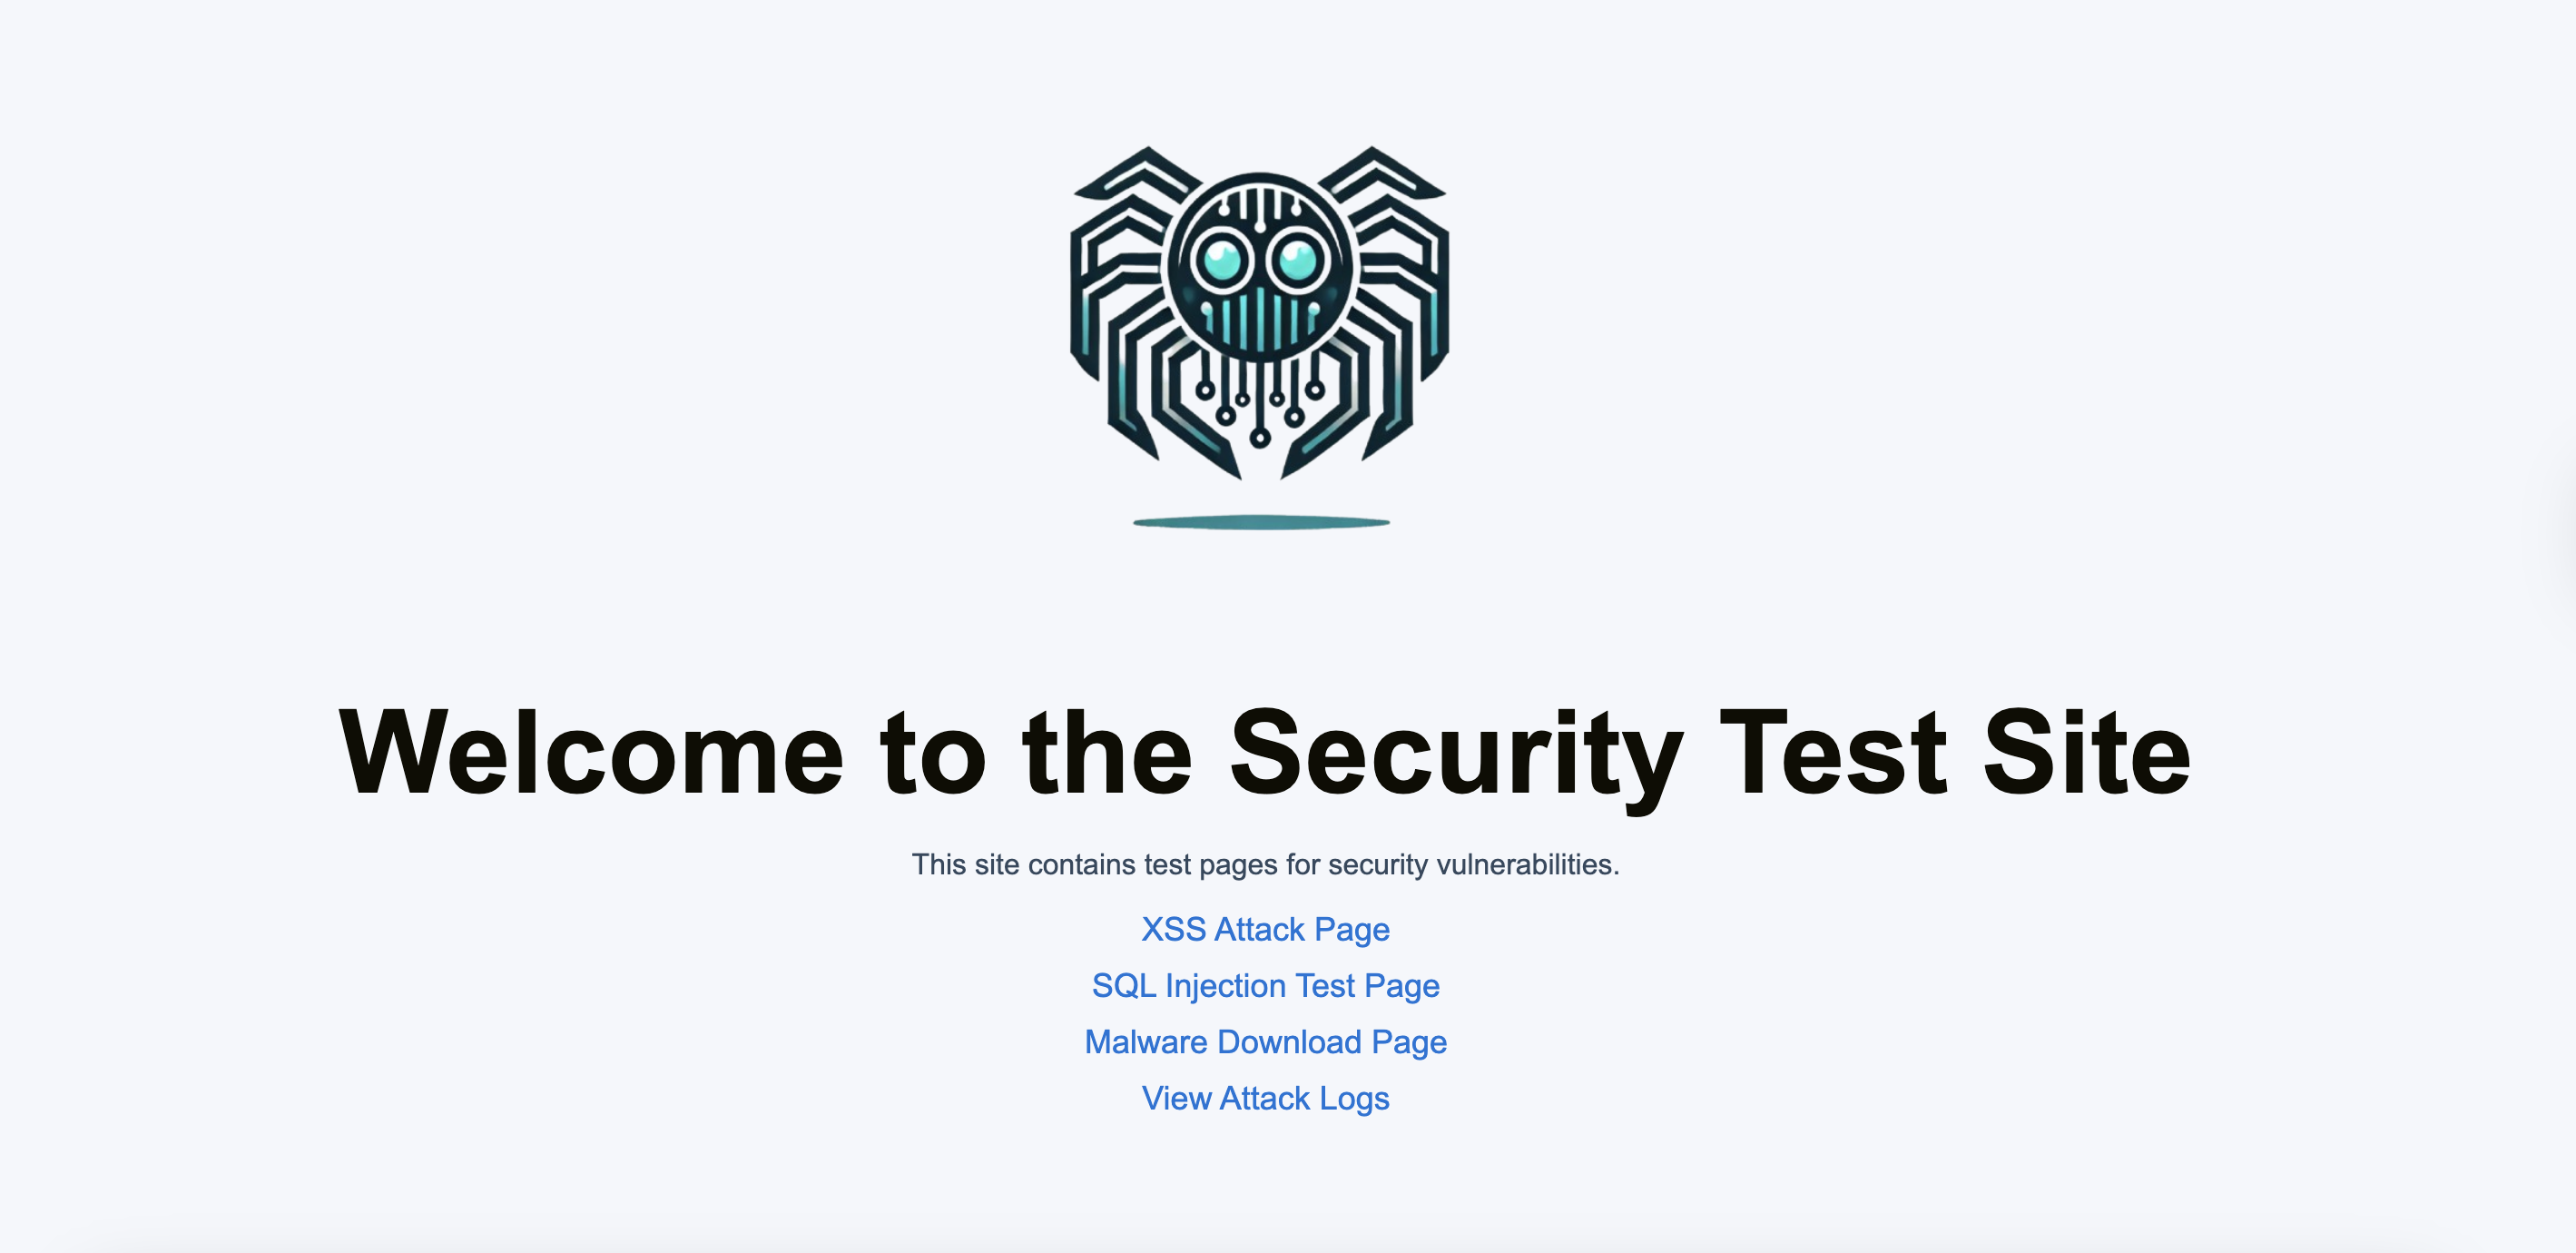
\includegraphics[width=\textwidth]{figures/home.png}
  \caption{Home Page}
  \label{fig:homeappendix}
\end{figure*}

\begin{figure*}[!t]
  \centering
  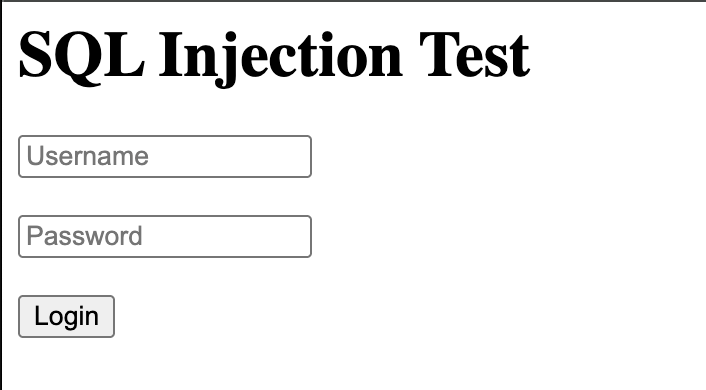
\includegraphics[width=\textwidth]{figures/sqltest.png}
  \caption{SQL Injection Test Site}
  \label{fig:sqltestappendix}
\end{figure*}

\begin{figure*}[!t]
  \centering
  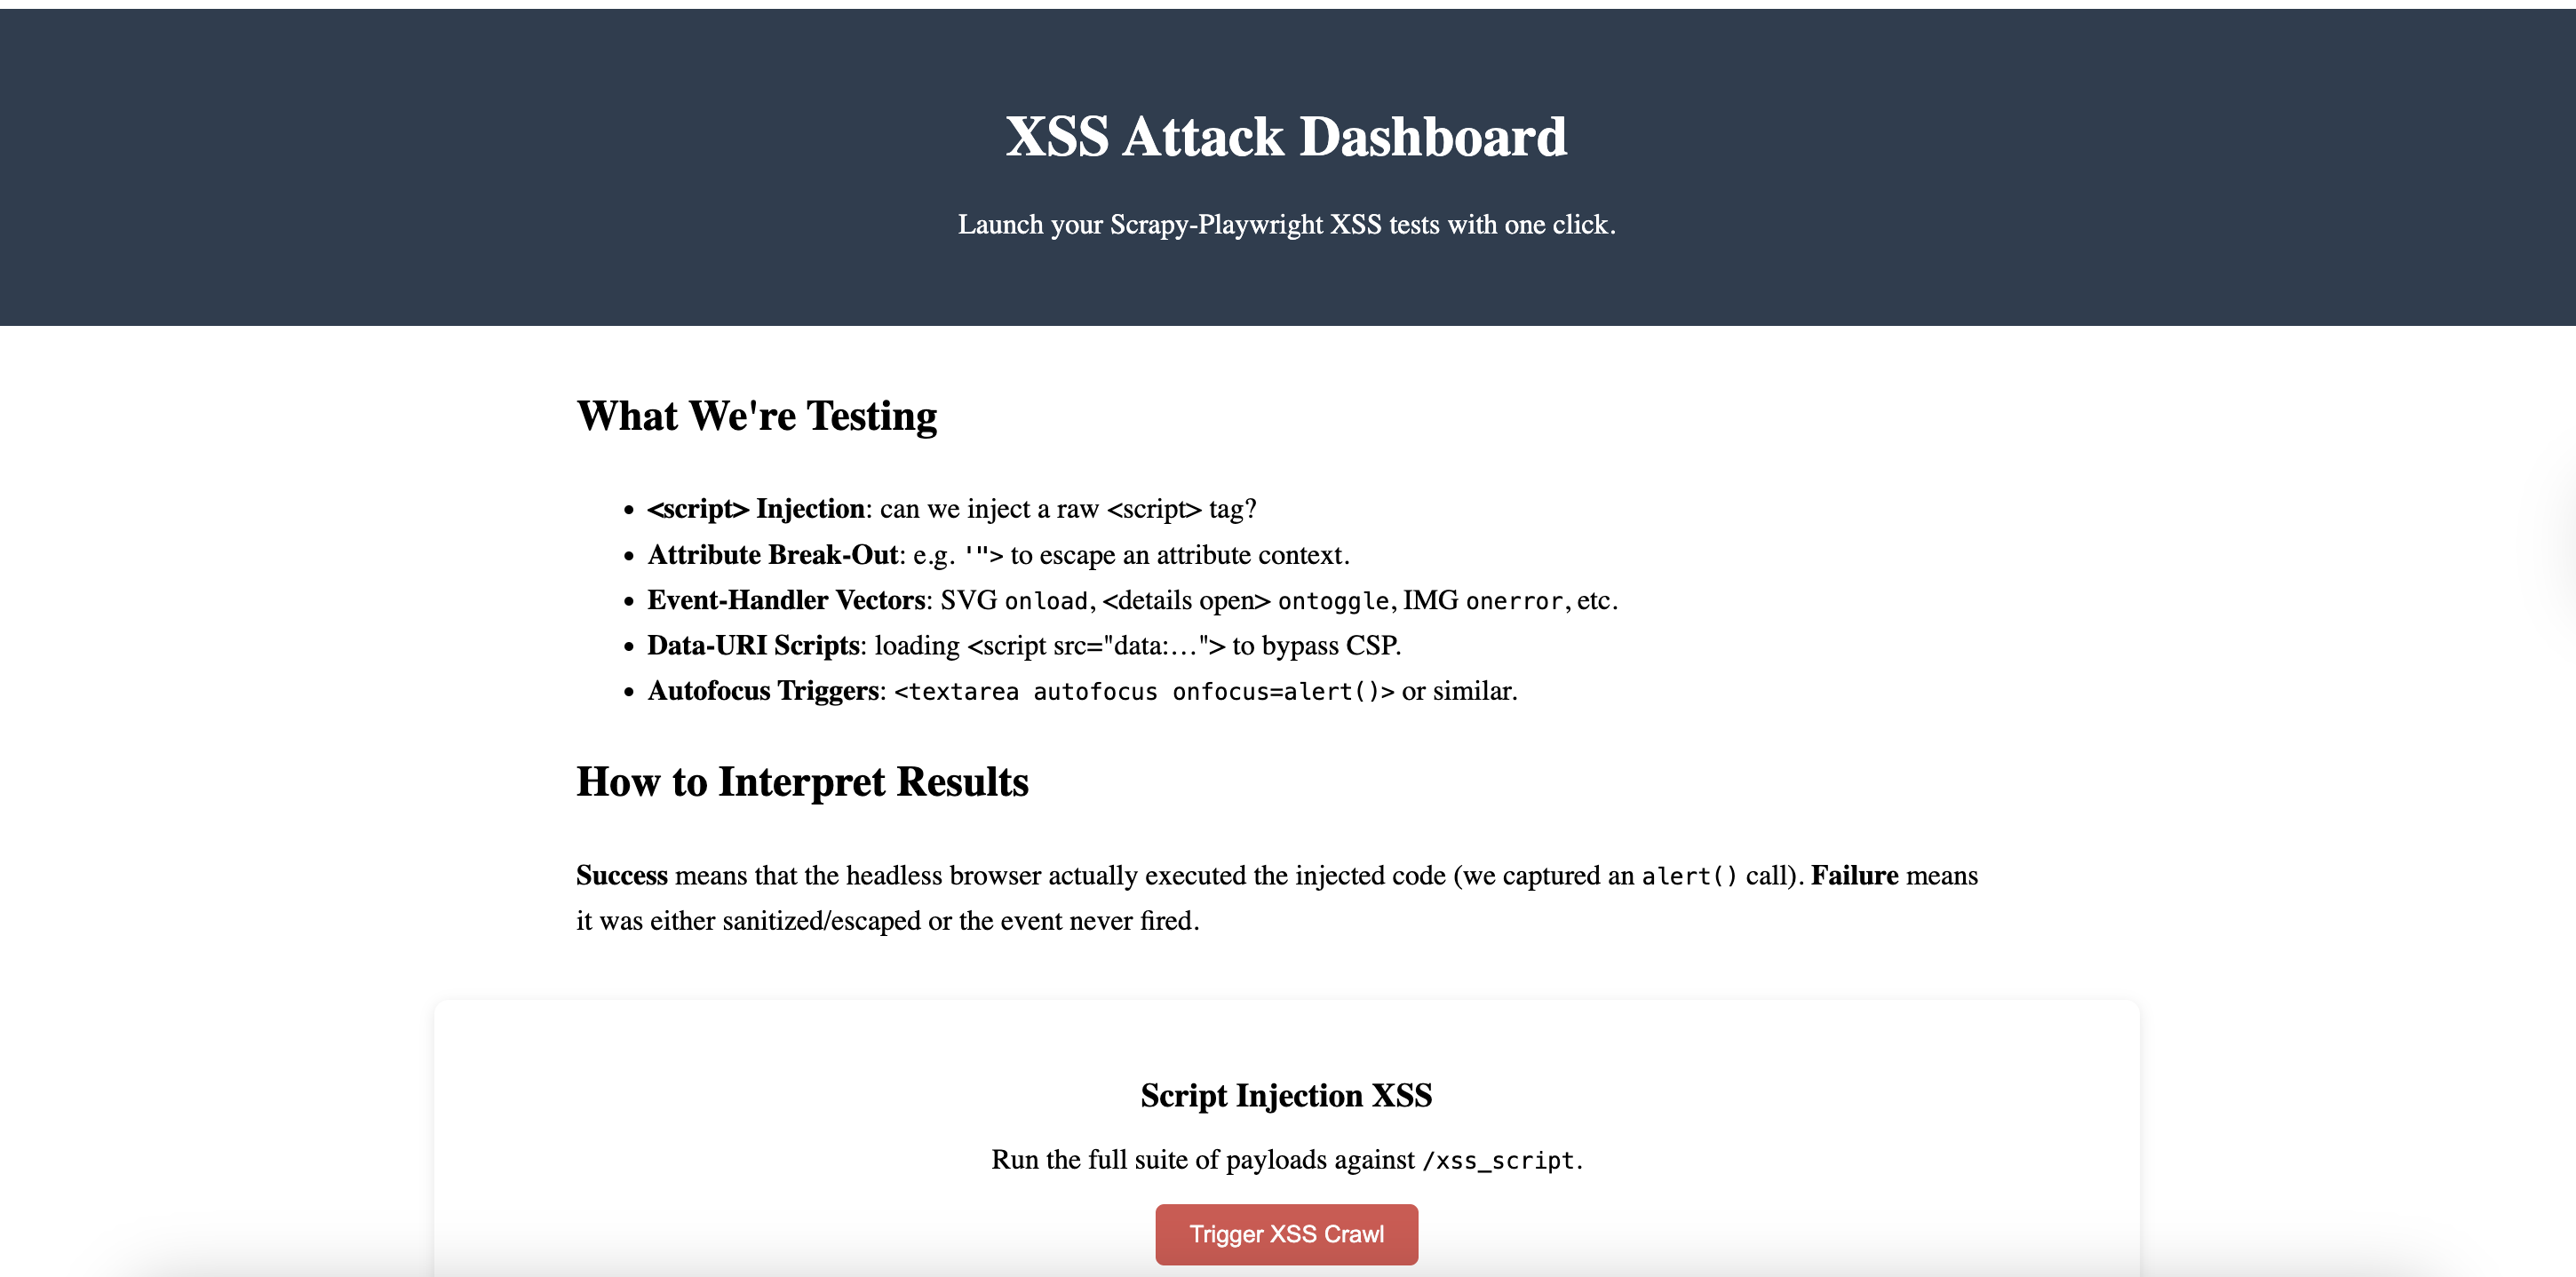
\includegraphics[width=\textwidth]{figures/xssdash.png}
  \caption{XSS Test Site}
  \label{fig:xssdashappendix}
\end{figure*}

\begin{figure*}[!t]
  \centering
  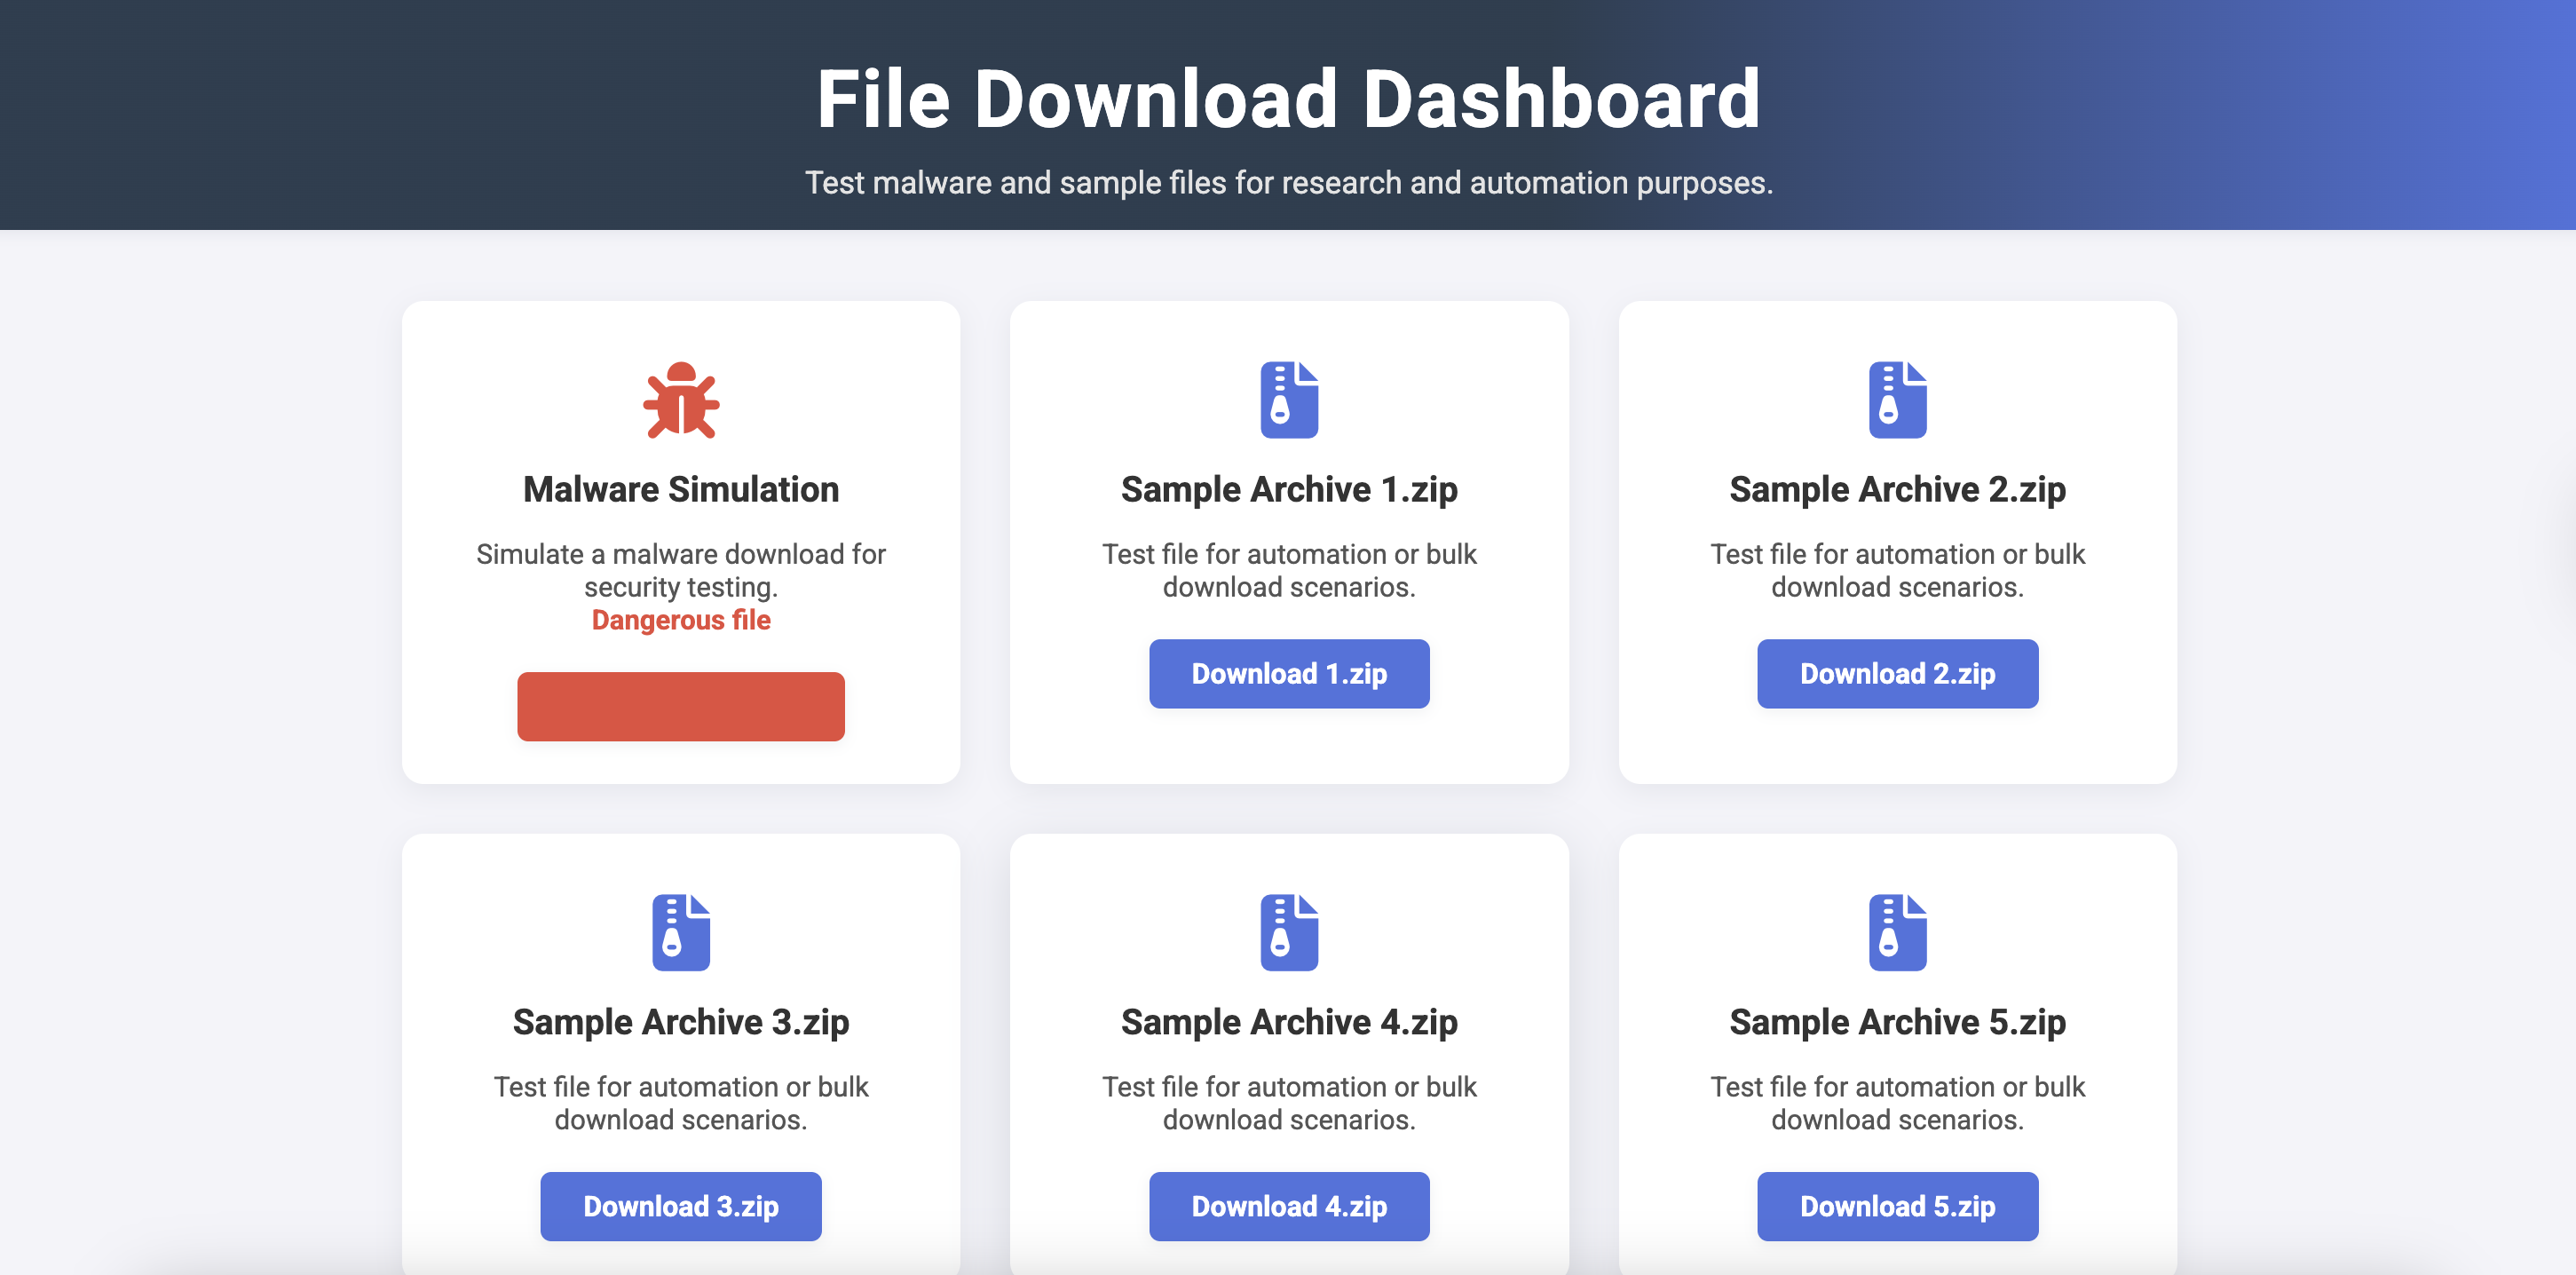
\includegraphics[width=\textwidth]{figures/maldash.png}
  \caption{Malware Download Test Site}
  \label{fig:maldashappendix}
\end{figure*}

\begin{figure*}[!t]
  \centering
  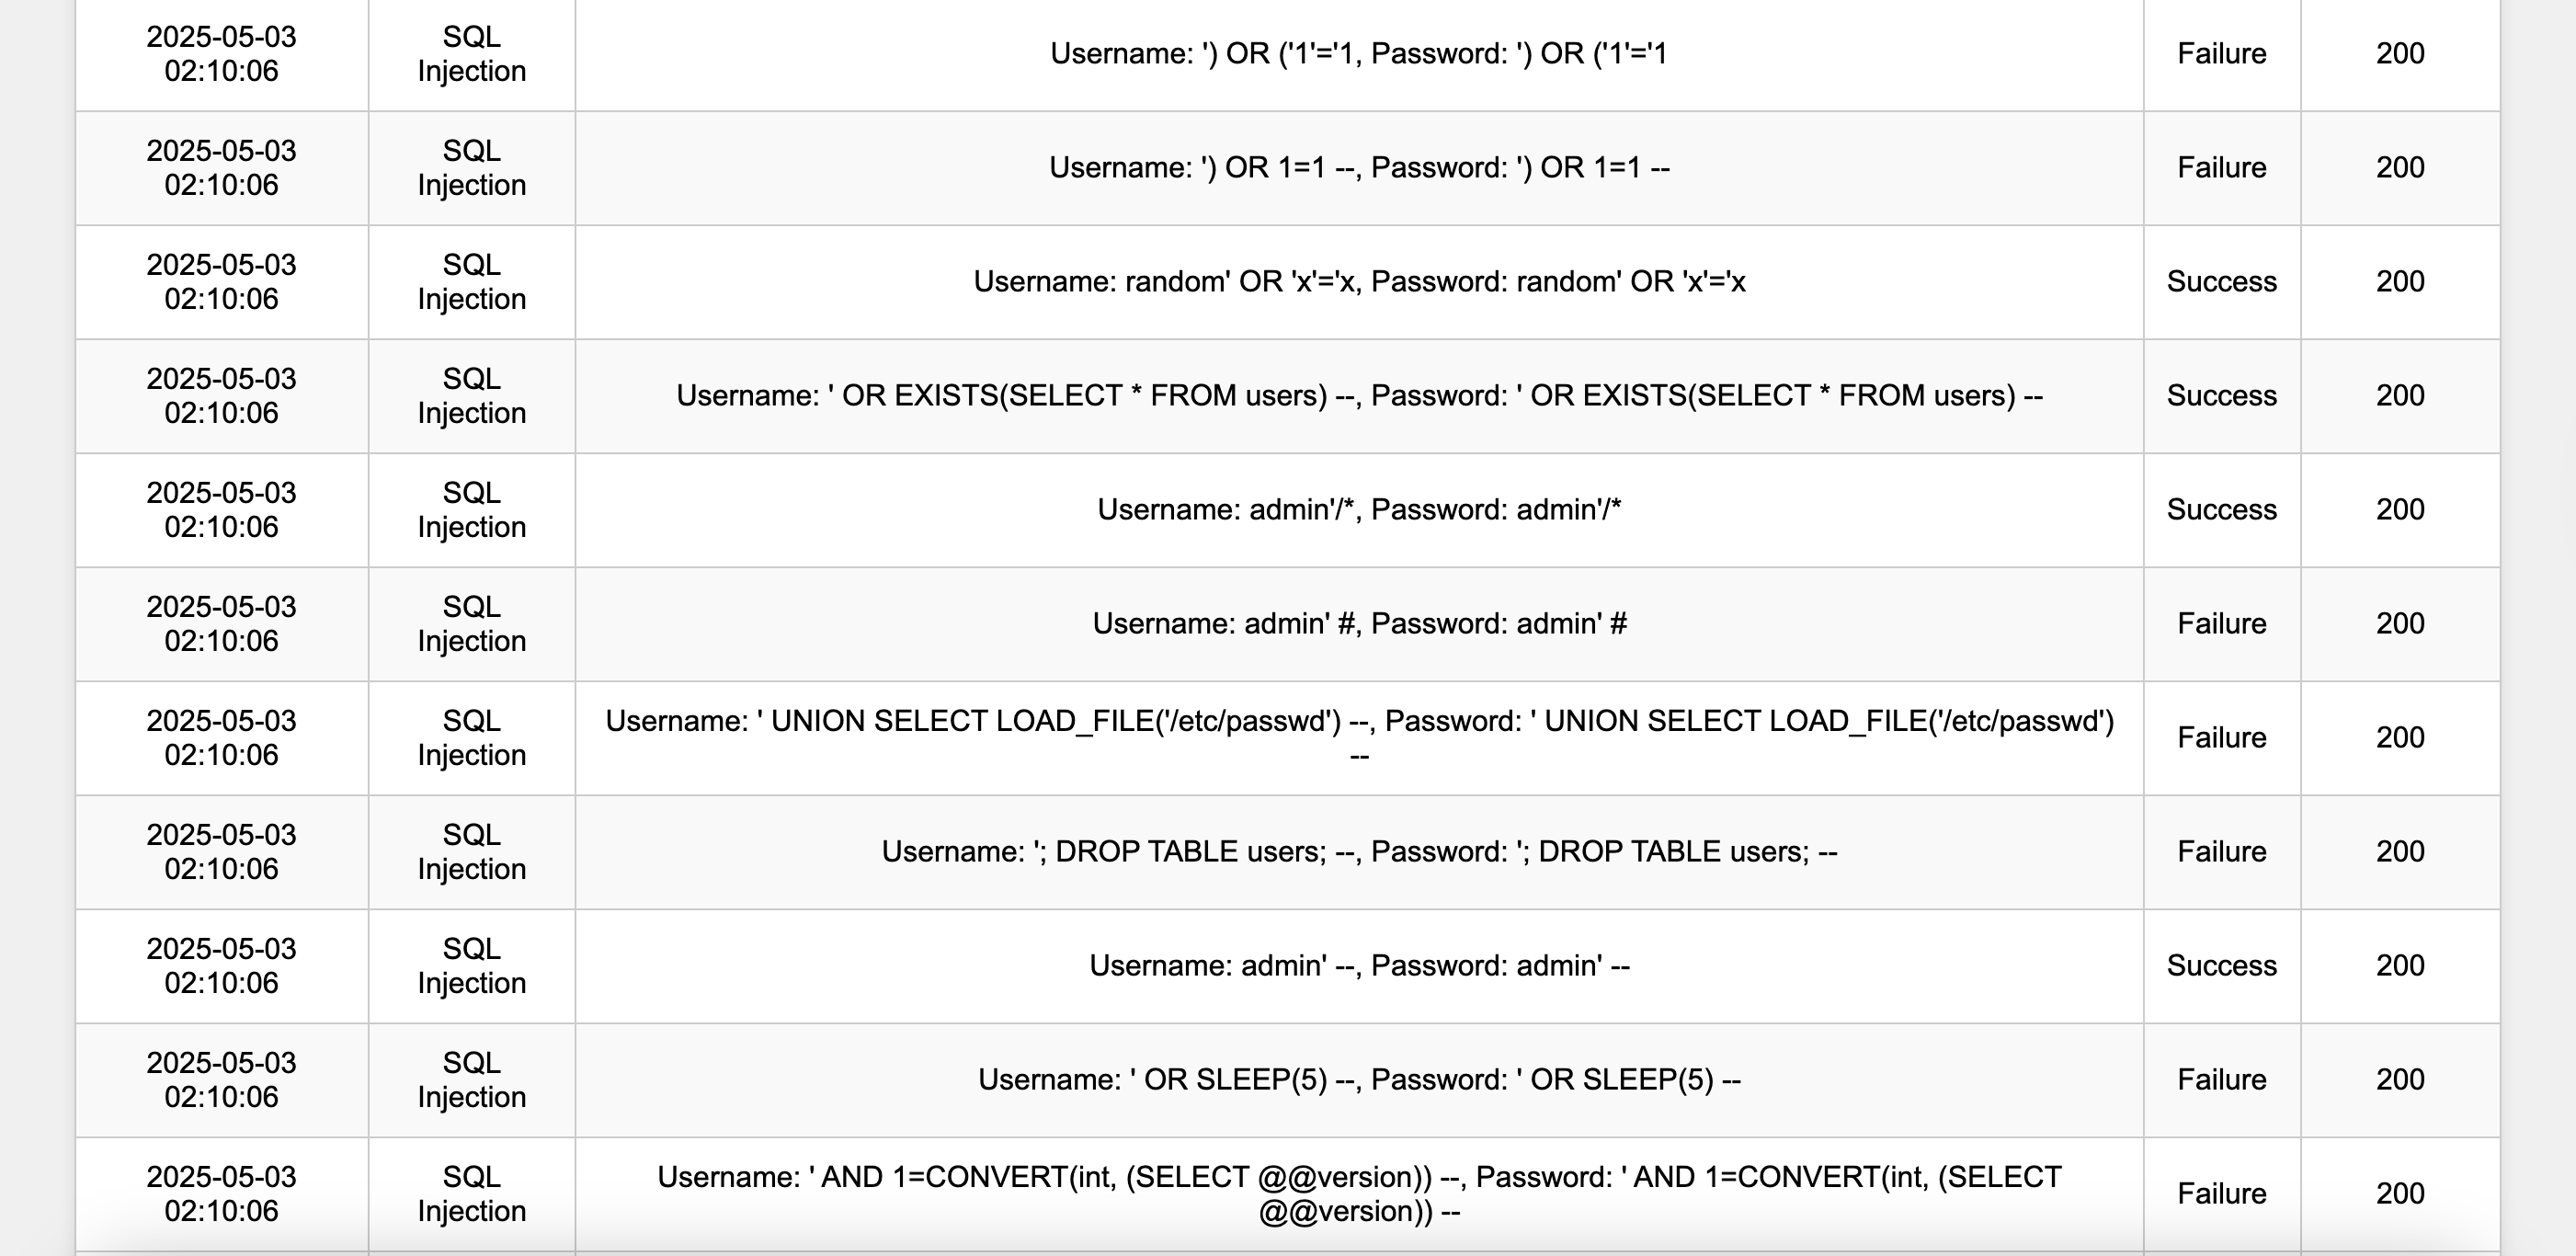
\includegraphics[width=\textwidth]{figures/sqli.png}
  \caption{SQL Injection Results}
  \label{fig:sqliresultsappendix}
\end{figure*}

\begin{figure*}[!t]
  \centering
  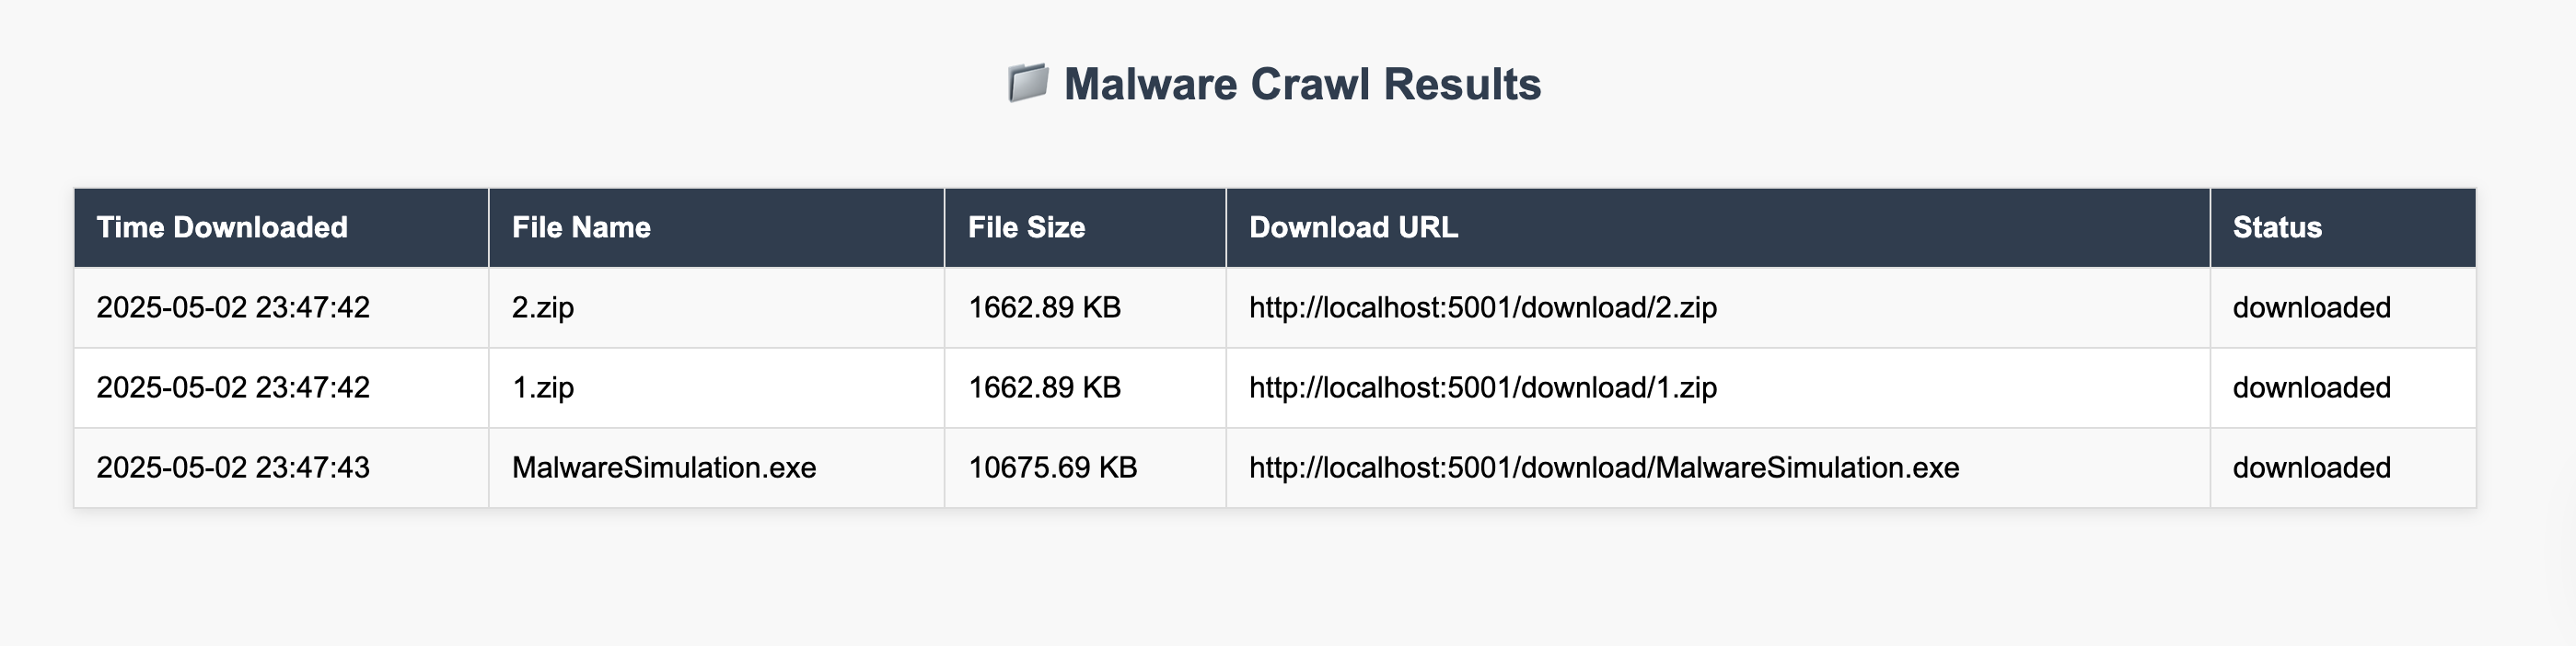
\includegraphics[width=\textwidth]{figures/malres.png}
  \caption{Malware Crawl Results}
  \label{fig:malresappendix}
\end{figure*}


\end{document}
